\documentclass[11pt, a4paper]{article}

\usepackage{geometry}
 \geometry{
 a4paper,
 total={210mm,297mm},
 left=25mm,
 right=25mm,
 top=30mm,
 bottom=25mm,
 headsep=7mm}

\usepackage{graphicx}
\usepackage{todonotes}
\usepackage[hidelinks]{hyperref}
\usepackage{listings}
\usepackage{enumerate}
\usepackage{fancyhdr}
\usepackage{longtable}
\usepackage{comment}
\usepackage{lipsum}


\graphicspath{ {images/} }

\pagestyle{fancy}
\fancyhf{}
\fancyhead[L]{\leftmark}
\fancyfoot[C]{\thepage}
\renewcommand{\headrulewidth}{0.4pt}

\begin{document}

	\begin{titlepage}
		\centering
		% logo image
		
\includegraphics[scale =0.8]{logo.jpg}\par\vspace{1cm}
		% institution 
		{\scshape\LARGE\bfseries Ecole Polytechnique de Louvain\par}
		\vspace{1.5cm}
		{\scshape\Large \par}
		\vspace{1.5cm}
		% title
		{\huge\bfseries LINGI2364: Mining Patterns in Data \par}
		\vspace{1cm}
		{\Huge Project 1: Implementing Apriori \par}
		\vspace{2cm}
		{\LARGE Group 11\par}
		% versioning
		\vspace{1cm}
		% author
		{\Large\itshape Alessandra Rossaro (01211800), Matteo Salvadore (01731800)\par}
		\vspace{2cm}
		{\small Version 1.0 - 21/10/2018\par}

		\vfill

		% Bottom of the page
		{\large AY 2018-2019\par}
	\end{titlepage}

	\section{Implementations}
		\subsection{Apriori}
			To implement the Apriori algorithm we have created ad hoc implementation of an HashTree that is used to contain the internal structure of the Apriori search. Every node of the HashTree is characterized with an HashMap containig its children nodes and the frequency of the node. 
			We have chosen this data structure in order to simplify the accesses of the algorithm to the elements of the SearchTree since the complexity of the access is $O(1)$.\newline
			Since the Apriori algorithm, in order to expand a new level, needs the previous one, during the Database reading process, we have saved in a TreeMap where the keys are all the patterns with a singular element and the values are the corresponding supports, computed incrementally during the reading process.\newline 
			This is the only improvement that we have performed on the \textit{DataSet} class that we have renamed into \textit{AprioriDataSet}.
			For the next levels the search is performed accordin to the Apriori algorithm specifications.
			\newline \newline
			We have then implemented the following optimizations:
			\begin{itemize}
				\item We generate candidates according to the \textit{Merging itemsets technique}: when we expand nodes to generate new candidates we take the nodes with same father of the node that is being expanded and we select as candidates only those have keys with value higher w.r.t. the current node's key.
				\item After the nodes generation we prune the infrequent candidates by computing their frequency. Those nodes are not considered for the new levels' expansion.
				\item Our HashTree data structure is implemented as a \textit{Prefix Tree} to make the merging more efficient, the order of the items in the tree is the natural Integer order.
			\end{itemize}
		\subsection{ECLAT}
			To implement the ECLAT algorithm we have redefined the \textit{DataSet} class into \textit{ECLATDataSet} class, since this algorithm needs to read database and to convert it into its \textit{Vertical Representation}.
			This new class loads the entire database in memory and then it creates the \textit{Vertical Representation} using a TreeMap that contains as key an Integer that represents a singular element and as value an HashSet of Integers that represent the numbers of transactions in which the singular element appears.
			We have decided to use this kind of data structure since just using an array to store the transaction numbers was inefficient. With our improvement the access complexity to insert an item in an HashSet is $O(1)$ and to access to the TreeMap is still $O(1)$.\newline
			This kind of data structure is used whenever the algorithm projects the Database on a new item.
			We have implemented the ECLAT algorithm following the specifications of \textit{Depth-First Search} algorithms explained in the slides of the course.
			\newline \newline
			We have implemented the following optimizations:
			\begin{itemize}
				\item As explained before, we have used an HashSet in our data structure to store the list of transaction numbers in which the singular item appears. Our decision was the result of a sequence of attempts to choose the most performant data structure: our first choice was an ArrayList that we have discarded because the execution time spent to transform the Database in the \textit{Vertical Representation} was too high, the same same problem occurred with our second choice: a vector of Integer.
				\item Thanks to the HashSet we can perform the intersection more efficiently since, instead of scanning two lists, we can just take the shorter list and search for the singular items in the longer one exploiting the fact that checking if an element is present in a HashSet is $O(1)$, then the total complexity of an intersection is $O(l)$ where \textit{l} is the length of the smaller HashSet.
				It is worth noting that comparing the shorter HashSet with the longer minimizes the number of comparisons to be performed.
				\item Before the computation of the intersections among a line of the \textit{Vertical Representation} and an item, we skip the computation with the Hashset with a support lower than minimum support. This is equivalent to the perform \textit{pruning} on the SearchTree.
			
			\end{itemize}
			
	\section{Performances}
		We have decide to use only the following datasets to compute the performances in terms of time and memory with different support values:
		\begin{itemize}
			\item \textit{chess.dat}
			\item \textit{mushroom.dat}
			\item \textit{pumsb.dat}
			\item \textit{pumsb\_star.dat}
			\item \textit{connect.dat}
			\item \textit{retail.dat}
			\item \textit{accidents.dat}
		\end{itemize}
		The datasets are ordered according to the ascending number of rows.
		\newline\noindent
		We have decided to discard \textit{toy.dat} because of its dimension: the results of the performances computed were inconsistent w.r.t. the overhead (in terms of memory occupied and elapsed time) by the JVM.
		\newline\newline
		\noindent
		The first computation of performances was with a range of values between 0.1 and 0.9, but we have noticed that already from the first data-set, for a frequency equal to 0.4, the running time was too high to be computed from our laptop.\newline
		For this reason we have decided to use a frequency that starts from 0.95 and to use a step of 0.05 and to run the performance script until the running time were too long; whenever we noticed that a data-set were taking too long for a specific frequency we have ignored it for lower frequencies.
		In the following sections, we have plotted the performances in terms of running times and used memory, w.r.t. different frequency values and for all data-sets. The running time graphs are plotted with axis that uses  logarithmic scale for the time.
		We have encountered some difficulties in measuring the memory usage of our Java application since the values obtained were not too much coherent between different executions with the same parameters and even forcing the garbage collector to flush the memory was not so useful to tamper this phenomenon; We've then tried to average the results of consequent runs to keep the measurement performances coherent.
		\subsection{Apriori}
			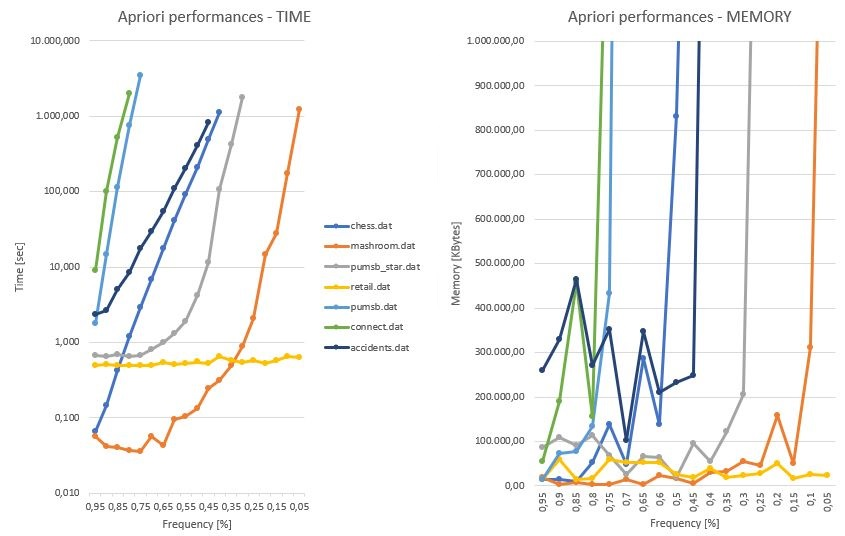
\includegraphics[scale =0.7]{Apriori.JPG}\par\vspace{1cm}
			As you can notice in the graph, the running time of our algorithm increases as the frequency decreases, for all data-sets, this kind of increase is exponential; for smaller data-sets this kind of phenomenon is acceptable (e.g. \textit{retail.dat}), while for data-sets with very long transactions and very similar transactions (e.g. \textit{connect.dat}) the running time increases more rapidly. \newline
			We have expected that \textit{accidents.dat} database would be way more time requiring w.r.t.the other data-sets, since it has the longest number of transactions but we have observed that the length of the transactions and the similarities of the transactions have more impact on the running time.
			We've noticed that the memory usage more or less grows as the frequency decrease and explodes at the same frequencies at which the running time exponential function begins to assume a very high slope (when it starts tending to infinite).
		\subsection{ECLAT}
			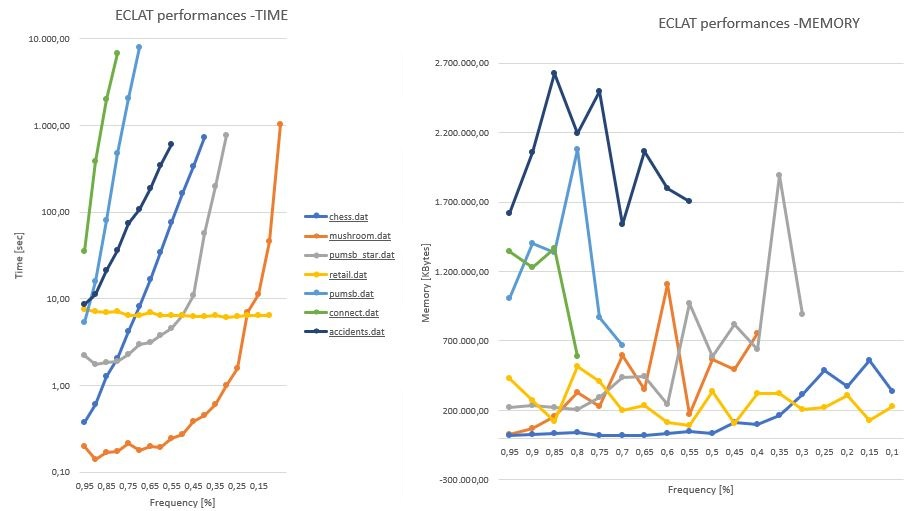
\includegraphics[scale =0.7]{ECLAT.JPG}\par\vspace{1cm}
			As you can notice in the graph, the behavior we have obtained with our implementation of ECLAT is very similar to the Apriori performances, but the exponential have a slightly smaller grow rate, and so their growth becomes very fast with slightly lower threshold of frequencies.
			An exception of this observation is that the data-set \textit{accidents.dat}, that has a way higher number of transactions probably has an higher impact on the performances due to the vertical representation usage in this algorithm, and so our ECLAT algorithm performances are worse w.r.t. Apriori for this specific data set.
			We have expected that the memory usage would have followed more or less the same behavior, but even with multiple measurements the behavior obtained is fuzzy, in particular all the data-sets at exception of \textit{connect.dat}, \textit{chess.dat} and \textit{accidents.dat}  we can make the same observations we have done with our Apriori algorithm, but we cannot explain the behavior of these three databases

\end{document}
